\chapter{Background}

\label{chap:background}
In this chapter, we introduce the concept of Wireless Sensor Networks. Moreover, we describe the Chaos and \atwo{} protocol in detail. Finally, we explain what clustering is and provide some insight into different objectives when applying clustering to a network, and also present clustering properties and their categories.


\section{Wireless Sensor Networks}
A \emph{Wireless Sensor Network} (WSN) consists of many low powered nodes (small computers) equipped with sensors, cooperatively working towards the same goal. Typical applications are within the military for tracking targets, monitoring the weather, and tracking natural disasters \cite{Yick2008-wsn-survey}. A typical node in a sensor network consists of four hardware units for sensing, processing, transmitting and receiving data, and power \cite{Akyildiz2002-wsn-survey}, there can also be additional units for generating power or sensing the location of the node. There are several characteristics of a WSN that while introducing challenges when working with them also are at the core of what makes them useful. Examples of these characteristics are the low power nature of the nodes and ad hoc deployment of the nodes.


One of the primary objectives of a node in a WSN is to preserve as much battery power as possible. Therefore the hardware is often limited in its capabilities, limiting both the radio communication range and the processing power \cite{NikolaosA.Pantaziz2007-wsn-power-survey}. An example of a node called TMote Sky \cite{tmotesky-datasheet}, which we use in this thesis, has a CPU of 8MHz, 10KB RAM, and 48KB of flash storage. The lifetime of the network can be measured in several different ways; one common way is to measure the time until the first node death occurs.

Another focus for the protocol a WSN is running is reliability. The network has to be able to handle a variety of failures such as: packet loss due to interference or transmission error, and nodes failing due to loss of battery power or other unforeseen errors \cite{Mahmood2015-reliability-survey}. In addition, if the network is multi-hop and nodes have to act as forwarders that can introduce several points of failure for a packet before it reaches its intended destination. There exist two primary categories of protocols when talking about how they handle reliability: retransmission and redundancy \cite{Mahmood2015-reliability-survey}. A protocol based on retransmission will have each node wait for acknowledgement of the packet it sends; otherwise, the node will retransmit the packet. A protocol based on redundancy, on the other hand, includes redundancy in the packet itself and will try to correct any faulty bits in any packets received.



\section{Chaos}
The Chaos protocol is the first protocol developed for WSNs that support native all-to-all communication without sequential phases for collection, processing, and dissemination of information \cite{chaos-introduction-paper}. Traditionally, every node in the network had to schedule these phases at the same time, even if some nodes did not have any information to process. In Chaos, every node can take independent decisions on what action to perform (send or receive data), but every node does their respective action at the same time, this is called synchronous transmissions.


The smallest time component in the Chaos protocol is called a \textit{slot}. During a slot, every node performs one of two actions: broadcast or listen for data. At the end of a slot, every node decides what their action will be in the next slot.
A node will broadcast in the subsequent slot if it receives a packet with less or more information than itself. In the first case, it tries to spread its information to the node which sent a packet with less information. In the other case, a node which has just received a packet which contains new information will merge this with their local data and then broadcast the new merged information in the next slot. If a node was listening, but either did not receive a packet or did not gain new information, or if it was broadcasting, then it will listen in the next slot. The next greater time component in Chaos is a series of many slots, and together they are called a round.

During one \textit{round} Chaos executes one application. For example, the max application in which all nodes spread their id across the network and the merge operator (the max application) executed on packet reception returns the maximum between the received number and a nodes local state. The number of slots in a round depends on the network size; a larger network requires more slots than a small network. We give an example of three nodes executing a round in  \cref{fig:chaos-overview}.

\begin{figure}[bt]
    \centering
    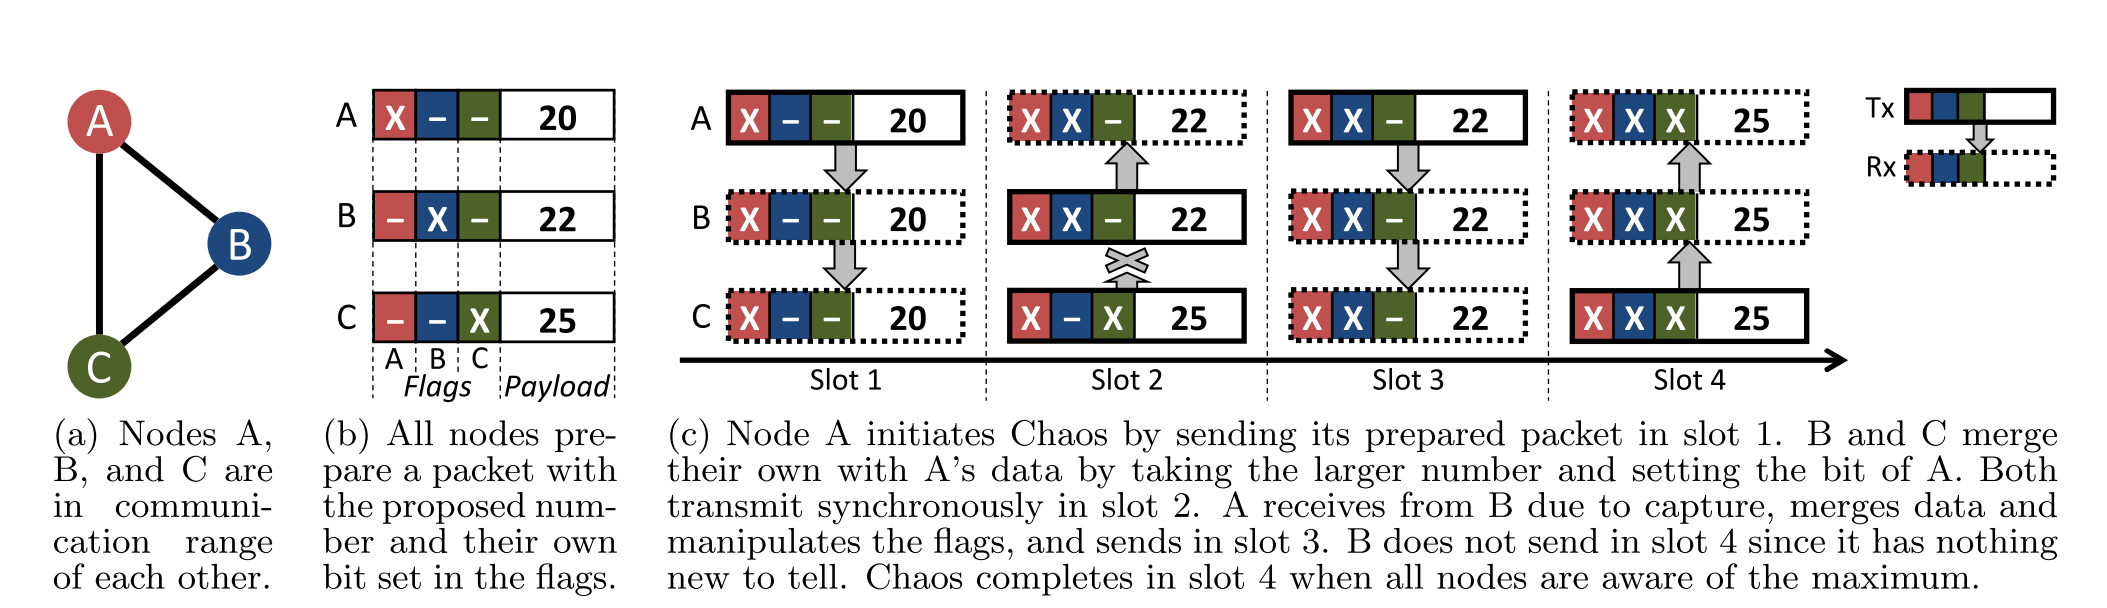
\includegraphics[width=\textwidth]{figure/ChaosOverview.png}
    \caption{Overview of a round in Chaos were three nodes try to reach consensus on a proposed value \cite{chaos-introduction-paper}.}
    \label{fig:chaos-overview}
\end{figure}

\subsection{Synchronous Transmission}
Using synchronous transmissions means that all nodes execute rounds and slots at the same time. In \cref{fig:chaos-overview} time progresses towards the right, and we see that all slots are aligned. This transmission scheme enables Chaos to benefit from two physical phenomena:

\paragraph*{The capture effect} is a physical phenomenon that occurs when packets are colliding (received at the same time by one node). If one signal is sufficiently stronger or the timing between the packets are within a certain threshold, a node will correctly decode the stronger signal, and ignore the weaker one \cite{Lee2007-capture-effect}. Due to this effect, if a node receives two transmissions at the same time, one of them will with a high probability be decoded correctly.

\paragraph*{Constructive Interference} is another physical phenomenon that occurs when multiple nodes are transmitting the same packet at the same time. If that happens, the radio signals get boosted increasing the probability that the packet will be received correctly by another node.

\subsection{The Initiator}
In every Chaos network a special node called \emph{the initiator} needs to be present, node \textit{A} in \cref{fig:chaos-overview}. First, the initiator is the node which initiates communication in a round. It also determines parameters such as what application to run and timing parameters for slots and rounds. All other nodes exclusively listen for packets until one is received which propagated from the initiator, this process is called association. A node will enter association when it boots up and if it does not receive a valid packet for a number of rounds that can be configured depending on the application that is running in the network. The initiator is a predetermined node.

\subsection{Flags Field}
\label{subsec-flags-field}
The \textit{flags field} is a list of boolean values. The field is marked as \textit{flags} in \cref{fig:chaos-overview}. Each node in the network corresponds to an index in the list. At the start of a round, the initiator only sets the value at its index to true. As packets propagate through the network, nodes set the value of their indices to true. Once a node has merged a received packet which sets all values in the flags field to true it knows that all nodes in the network have participated and the information it has is complete. The Chaos protocol has a limitation to its scalability due to the flags field. Since every node requires at least a 1-bit space in the flags field, if there is an upper limit on the packet size imposed by either the link-layer protocol or the sensor nodes, the number of nodes in the network is limited by the maximum size of the packet. 

\subsection{Completion Flooding} % The chaos papers call it the completion policy, they also have the propagation policy as "normal" mode
\emph{Completion flooding} is the last phase of a round. A node enters this phase as soon as all values in their flags field are set to true. Once in this phase, the node broadcasts its completed packet every other slot for a number of slots. Aggressively transmitting the packet causes neighbouring nodes to reach completion which in turn causes them to flood the network with a completed packet. Since all nodes in this phase broadcast the same packet the signal benefits from constructive interference which in turn makes the signal of the complete packet stronger causing the capture effect to apply more often.

\subsection{Timeout Mechanism}
To prevent early termination a \textit{timeout mechanism} triggers if a node has not received any packet for some number of slots. Early termination is when, at the end of a round, some nodes do not have all information. The number of slots is selected randomly by each node from an interval ([3-7] in \cite{chaos-introduction-paper}) causing one or a couple of nodes to broadcast a packet. If nearby nodes have non-equal flag fields, they will continue the packet propagation, and thus communication is reinitiated.

\section{\atwo{} Synchrotron}
\label{sec:chaos-a2-background}
As the original implementation of Chaos has lots of potential, further research conducted by Al Nahas et al.~\cite{a2-introduction-paper} resulted in the Agreement in the Air (\atwo{}) Synchrotron.
As seen in \cref{fig:original-a2-architecture}, \atwo{} is a layer on top of Synchrotron, which is a further development of Chaos. Synchrotron's most prominent features and the ones described here include a dynamic scheduler, parallel channels and channel hopping. From \atwo{} we describe the join and leave services. The remaining architecture description shown in \cref{fig:original-a2-architecture} is explained in \cite{a2-introduction-paper}.

\begin{figure}[bt]
    \centering
    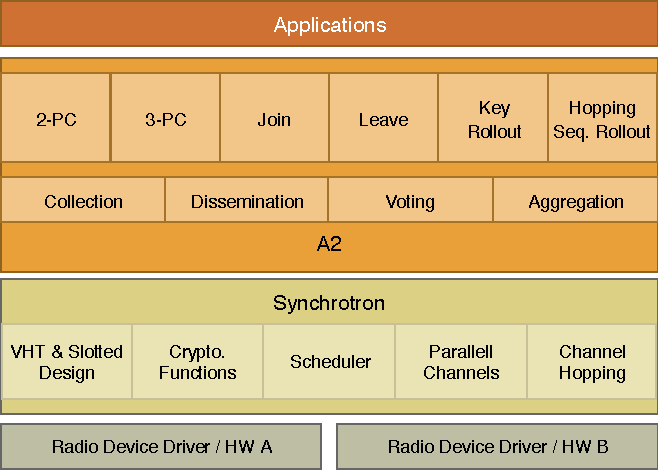
\includegraphics[scale=0.7]{figure/architecture_original_a2.pdf}
    \caption{The original \atwo{} architecture \cite{a2-introduction-paper}.}
    \label{fig:original-a2-architecture}
\end{figure}

The second contribution is a voting primitive which is used to implement distributed consensus algorithms and a consistent group membership service. 

(include an example of how A2 runs, dynamic join service then application)

\subsection{The Scheduler}
The scheduler in \atwo{} allows the initiator to schedule different applications dynamically. During each round, the initiator sets a \textit{next app} field in the packet to instruct the rest of the network which app should run in the next round.

\subsection{Dynamic Group Membership}
\label{background-a2-join-service}
The join service allows the network to add nodes to the flags field dynamically. A node wanting to join the network sets the join flag in the packet header. Once the initiator receives a packet with a set join flag, it will, during the next round, spread the scheduling of a join round for the subsequent round. The join round then runs in two phases, collect and disseminate. We show an example of the join process with three nodes in \cref{fig:join-service-overview}.

\begin{figure}[bt]
    \centering
    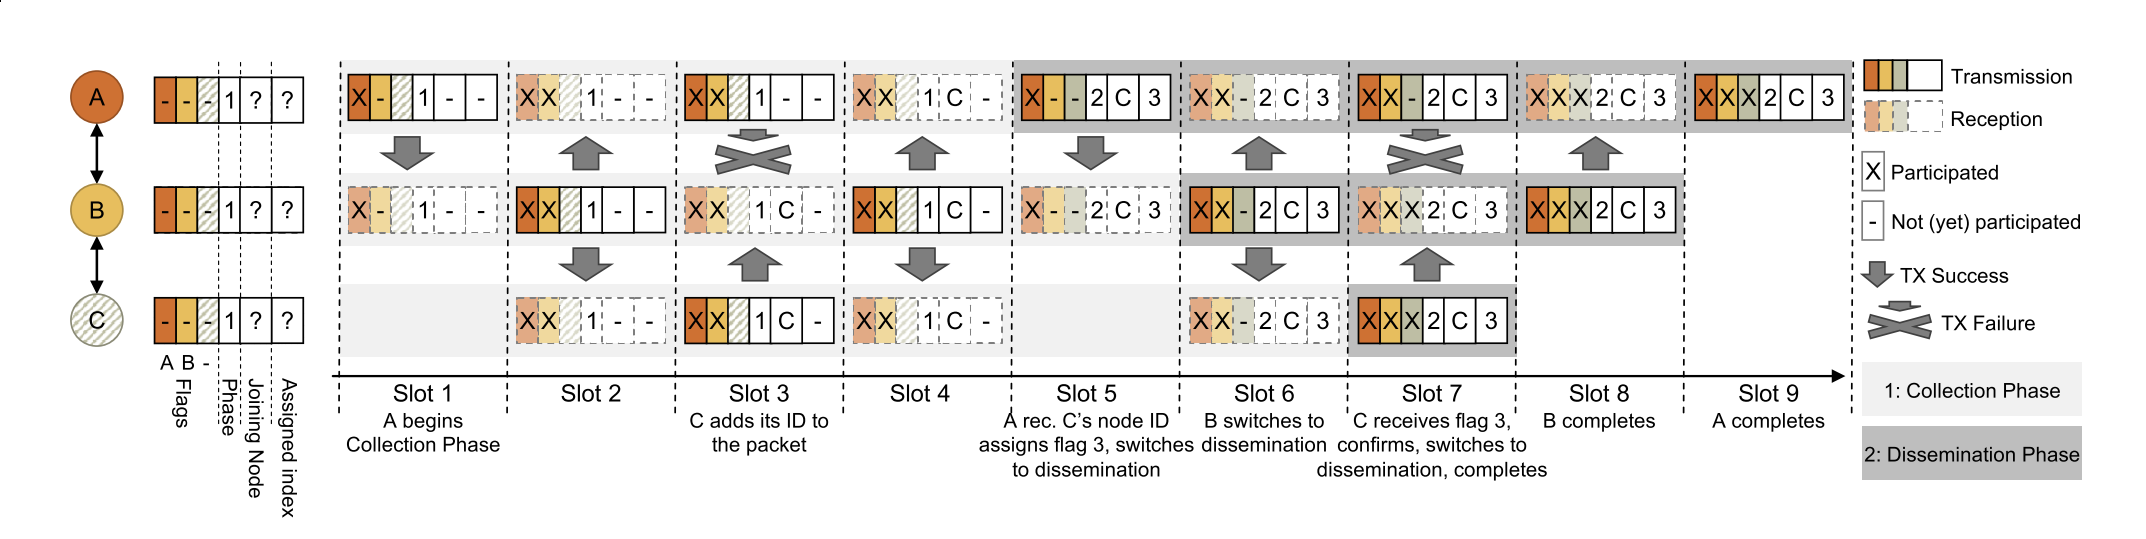
\includegraphics[width=\textwidth]{figure/JoinServiceOverview.png}
    \caption{The join service protocol exemplified using three nodes \cite{a2-introduction-paper}.}
    \label{fig:join-service-overview}
\end{figure}

\paragraph*{The Collect Phase} is the first phase where the network spreads a list in which nodes that want to join the network adds their node ID; this join list is the only way non-joined nodes may contribute to the payload. The initiator will switch to the next phase (Slot 4-5 in \cref{fig:join-service-overview}) when it notices full participation of the network and does not record any changes to the join list for a couple of slots or if the list is full.

\paragraph*{The Disseminate Phase} is the second phase where the initiator assigns each new node an index in the flag field. The initiator then disseminates the join list with updated information about the joining nodes flag indices. Each joining node can now set the flag in their specified index as an acknowledgement (C sets its flag in Slot 7). In case a node misses the dissemination it will requests another join round and be assigned the same flag index again.

The leave service is a rule that the initiator will drop any nodes which it has not seen participation from for a couple of rounds. When the rule triggers, a join round is scheduled to disseminate the information about what nodes are present. The leave service ensures that disappearing nodes does not hinder the completion phase for more than a small number of rounds.

\subsection{Frequency Agility}
\label{subsec-frequency-agility}
In the presence of interference, the performance of \atwo{} degrades. Al Nahas et al.~solves this in Synchrotron by introducing frequency hopping and parallel channels.

\paragraph*{Frequency hopping} in Chaos consists of each node switching which radio channel they use to transmit and receive data in unison in every slot. By switching channels, using the default hopping sequence from the IEEE 802.15.4e standard \cite{IEEE-802-15-4}, the network avoids interference from other traffic, which might occupy a single channel, allowing \atwo{} to exists side-by-side other wireless systems. 

\paragraph*{Parallel Channels} alleviates the issues caused by having a dense network with many nodes transmitting simultaneously in the same area. This causes interference which damages the probability of packet capture. Synchrotron allows for configuring a number of channels from which nodes pick randomly in each slot to use for reception or transmission. The number of parallel channels require configuration and could damage the performance of a network if it is set to high or low. An alternative to parallel channels, proposed by Landsiedel et al., is to reduce the transmission power which would also reduce network density.


\section{Clustering}
\label{sec:background:clustering}

In this section, we cover the topic of clustering. We begin with a high-level description of what clustering in a WSN means. Next, we describe the objectives desired when clustering a WSN. Finally, we describe categories for clustering properties as well as explain the properties that are important for understanding our work.

\subsection{High-level Description}
Clustering is the task of partitioning a network and electing particular nodes, called Cluster Heads (CH), responsible for a network-wide communication overlay \cite{Younis2006-clustering-survey}. All other nodes only communicate within their part of the partition, i.e., their cluster. Each cluster contains one CH which retains all information from the cluster. A typical use case is that all sensor nodes collect data and sends it to a \textit{base station}. A base station is not a sensor node, for example, it is not battery powered and only collects data from other nodes. In some networks, there is no base station; the aim is instead to inform all nodes in the network of the calculated values. In either case, it is the job of the CH to make sure that the relevant parties get the final value.

Related to base stations is the hot spot problem which is a phenomenon that can occur when nodes or cluster heads are using a many-to-one communication pattern \cite{Perillo2005-hot-spot-survey}. Nodes that are closer to the base station will need to handle more routing of traffic, and this can lead to them depleting their energy earlier than other nodes in the network. In the worst case, this can cause the network to become cut off from the base station entirely, completely disabling the network.

Clustering can be beneficial in several aspects; we list some objectives of clustering in \cref{sec:clustering-objectives}. One of the most critical components of a WSN is its energy consumption and using the radio to transmit and receive data is generally the most expensive operation of a node \cite{Anastasi2009-wsn-energy-consumption}. Clustering has been shown to decrease the energy consumption, making clustering an excellent candidate to preserve energy in a WSN.



\section{Clustering Objectives}
\label{sec:clustering-objectives}
There are two categories of clustering objectives, primary and secondary. When designing a clustering algorithm achieving one or more of the primary objectives is often the goal. In contrast, the secondary objectives are usually not of substantial importance for the network, but instead indirectly achieved when clustering the network \cite{Afsar2014-clustering-survey}. We list some primary and secondary objectives in \cref{table:clustering-objective}.

\begin{table}[bt]
\centering
\caption{An overview of primary and secondary clustering objectives \cite{Afsar2014-clustering-survey}.}
\label{table:clustering-objective}
\begin{tabular}{cc}
\multicolumn{2}{c}{{\textbf{Clustering Objectives}}}                   \\ \hline
\multicolumn{1}{c|}{\textbf{Primary}}            & \textbf{Secondary}      \\ \hline
\multicolumn{1}{c|}{Scalability}                 & Increased connectivity  \\
\multicolumn{1}{c|}{Fault-tolerance}             & Reduced routing delay   \\
\multicolumn{1}{c|}{Data aggregation/fusion}     & Collision avoidance     \\
\multicolumn{1}{c|}{Load balancing}              & Using sleep schemes \\
\multicolumn{1}{c|}{Stabilised network topology} &                         \\
\multicolumn{1}{c|}{Maximal network lifetime}    &                        
\end{tabular}
\end{table}

\subsection{Primary Clustering Objectives}
All the primary objectives are usually desired when implementing a clustering algorithm. However, it can be difficult to achieve all of them at the same time. Instead, it is common to target only a few of them.

\paragraph*{Scalability} is a consequence of clustering since the network is partitioned, making the network artificially less dense. Factors which we need to consider when designing for scalability include network density and routing delays.

\paragraph*{Fault tolerance} is common for mission-critical applications. A clustering algorithm can be fault tolerant by periodically reclustering the network. If a node dies and some part of the network loses connectivity, a reclustering can reconnect the network again.

\paragraph*{Data aggregation/fusion} is the act of filtering out redundant data at some earlier point. If the application of a WSN is running is only interested in some average or otherwise redundant data is sent the CH can filter out this data and decrease the number of packets transmitted. Clustering is known to reduce the total network load \cite{Afsar2014-clustering-survey}.

\paragraph*{Load balancing} is achieved by periodically changing the nodes that are CHs. Assuming that being a CH requires more battery, this will increase the total lifetime of the network when clustering is applied.

\paragraph*{Stabilised network topology} concerns the mobility of nodes. If a node moves and switches cluster, the CH can register this change and keep the network topology up to date.

\paragraph*{Maximal network lifetime} is a very common objective often, in part or entirely, caused by the other objectives. For example, proper load balancing means avoiding early node deaths, and data aggregation mean the network can send fewer packets. Both of these properties work towards an energy efficient cluster which implies a more extended network lifetime. 

\subsection{Secondary Clustering Objectives}
The secondary objectives are not usually a target when implementing clustering algorithms but rather achieved indirectly or enabled by them.

\paragraph*{Increased connectivity,} in a clustered network only the CHs needs to be connected to each other. All other nodes only have to be connected to their cluster which makes it easier to make the network fully connected.

\paragraph*{Reduced routing delay,} some applications may require a minimum routing time to perform as intended for example applications recording physical events such as earthquakes. To have a proper quality of service packets need to arrive within a specified time limit. In a widespread WSN, this can be a challenge.

\paragraph*{Collision avoidance,} transmission collisions may cause packet loss which is energy wasted on doing nothing. To minimise packet loss clusters can split their communication between different radio channels or different time slots.

\paragraph*{Using sleep schemes,} in some applications there is no need for the whole network to be active. For example, some nodes might only provide routing paths, in this case, all paths need not always be active. Thus, enable routing to work longer without any node deaths.


\section{Clustering Technology Properties}
\label{subsec:background:clustering-algorithm-categorisation}

There exist several ways of categorising the properties that define clustering algorithms. Afsar et al.~\cite{Afsar2014-clustering-survey} describe three main categories: Cluster properties, Cluster Head properties and Clustering process properties. Here, we summarise each category and list the properties within each of them.

\subsection{Cluster Properties}
The \textit{cluster properties} summarised in \cref{table:cluster-properties} describe properties of the clusters the algorithm creates.

\paragraph*{The size of clusters} in a WSN can either be tailored by the algorithm to be equal or unequal. In an equal clustering algorithm the algorithm will enforce an equal size on all clusters while in an unequal algorithm the clusters will vary in size according to some criteria, for example, distance to a base station; if a cluster is closer to a base station, the cluster size will be smaller.

\paragraph*{The number of clusters} can either be predefined or variable. When the cluster size is variable, it would be due to a probabilistic CH election process.

\paragraph*{The communication distance} can be either \textit{single-hop} or \textit{multi-hop} communication for both \textit{intra-cluster} and \textit{inter-cluster communication}. Inter-cluster requires multi-hop communication when the number of CHs are few and spread out since they will need help with forwarding to reach the other CHs. Intra-cluster communication needs to be multi-hop when there is a bound on the number of CHs since every node might not be able to reach a CH in a single hop.

\begin{table}[bt]
\centering
\caption{Cluster properties and their options.}
\label{table:cluster-properties}
\begin{tabular}{cl}
\multicolumn{2}{c}{\textbf{Cluster Properties}}                                                                         \\ \hline
\multicolumn{1}{c|}{\textbf{Property}}           & \multicolumn{1}{c}{\textbf{Options}}                                 \\ \hline
\multicolumn{1}{c|}{Cluster size}                & \begin{tabular}[c]{@{}l@{}}Equal\\ Unequal\end{tabular}              \\ \hline
\multicolumn{1}{c|}{Cluster count}               & \begin{tabular}[c]{@{}l@{}}Constant (preset)\\ Variable\end{tabular} \\ \hline
\multicolumn{1}{c|}{Intra-cluster communication} & \begin{tabular}[c]{@{}l@{}}Single-hop\\ Multi-hop\end{tabular}       \\ \hline
\multicolumn{1}{c|}{Inter-cluster communication} & \begin{tabular}[c]{@{}l@{}}Single-hop\\ Multi-hop\end{tabular}      
\end{tabular}
\end{table}

\subsection{Cluster Head Properties}
The cluster head properties listed in \cref{table:cluster-head-properties} define different behaviours for the cluster heads.

\paragraph*{The mobility} of a node is either mobile or stable. A mobile CH induces frequent topology changes which add overhead.

\paragraph*{The node type} is either homogeneous or heterogeneous. An algorithm with heterogeneous nodes means a node could have additional resources such as elevated energy reservoir, computing power or transmitting range. Making it more suitable to be CH than other nodes.

\paragraph*{The role} of a CH is either only to relay messages or to both relay messages and perform the same operations regular nodes do, such as collecting and aggregating data.

\begin{table}[bt]
\centering
\caption{Cluster head properties and their options.}
\label{table:cluster-head-properties}
\begin{tabular}{cl}
\multicolumn{2}{c}{\textbf{CH Properties}}                                                                    \\ \hline
\multicolumn{1}{c|}{\textbf{Property}} & \multicolumn{1}{c}{\textbf{Options}}                                  \\ \hline
\multicolumn{1}{c|}{Mobility}          & \begin{tabular}[c]{@{}l@{}}Mobile\\ Stationary\end{tabular}          \\ \hline
\multicolumn{1}{c|}{Node types}        & \begin{tabular}[c]{@{}l@{}}Homogeneous\\ Heterogeneous\end{tabular}  \\ \hline
\multicolumn{1}{c|}{Role}              & \begin{tabular}[c]{@{}l@{}}Relay\\ Aggregation/Fusion\end{tabular}
\end{tabular}
\end{table}

\subsection{Clustering Process Properties}
The clustering process describes the properties used to create the cluster, these properties are often more high level and describe the process as a whole.

\paragraph*{The method} used for clustering can be either distributed or centralised. A distributed algorithm has the potential to create clusters faster since each node can make its own decision. However, a centralised approach can create more optimised clusters since it has a global view of the network.

\paragraph*{CH election} can either be preset, random or attribute based. Preset is when the person who configures the network chooses which nodes are cluster heads during setup. The opposite of a preset approach is a random approach, letting the nodes become cluster heads with a probability. As a middle road, nodes may select CHs with a more complicated process using attributes such as remaining energy or the number of neighbours.


\paragraph*{The algorithm complexity} is either constant or variable. A constant complexity means setup time is not dependent on network size while a variable time algorithm can converge on better choices for cluster heads. 

\paragraph*{The nature} of the clustering process can either be proactive or reactive. Proactive means that it does not consider what application will run on it. In contrast, the process's nature can also be reactive or data-centric meaning it tries to optimise the cluster for a specific application and the data flow required by it.

\paragraph*{The dynamism} of the algorithm can be either dynamic or static. In a dynamic approach, CHs are elected based on the current conditions of the network while a static approach would yield the same result no matter when the algorithm executes.


\begin{table}[bt]
\centering
\caption{Clustering process properties and their options.}
\label{table:clustering-process-properties}
\begin{tabular}{cl}
\multicolumn{2}{c}{\textbf{Clustering Process}}                                                                       \\ \hline
\multicolumn{1}{c|}{\textbf{Property}}    & \multicolumn{1}{c}{\textbf{Options}}                                      \\ \hline
\multicolumn{1}{c|}{Method}               & \begin{tabular}[c]{@{}l@{}}Distributed\\ Centralised\end{tabular}         \\ \hline
\multicolumn{1}{c|}{CH election}          & \begin{tabular}[c]{@{}l@{}}Preset\\ Random\\ Attribute based\end{tabular} \\ \hline
\multicolumn{1}{c|}{Algorithm Complexity} & \begin{tabular}[c]{@{}l@{}}Constant\\ Variable\end{tabular}               \\ \hline
\multicolumn{1}{c|}{Nature}               & \begin{tabular}[c]{@{}l@{}}Proactive\\ Reactive\end{tabular}              \\ \hline
\multicolumn{1}{c|}{Dynamism}             & \begin{tabular}[c]{@{}l@{}}Dynamic\\ Static\end{tabular}                  \\ \hline
\multicolumn{1}{c|}{Objectives}           & See table \ref{table:clustering-objective}                                                       
\end{tabular}
\end{table}